\chapter{State of the art} \label{sec.state_of_art}

As the topic of this thesis is rather specific, comparable research is hard to find. Overall, the thesis works on the two subjects of unsupervised pre-training for \glspl{nn} and for \gls{ml} supported \gls{nids}. Here we are looking at state-of-the-art research of both aspects individually.

\section{Self-supervised Pre-training for LSTMs and Transformer Networks}

When it comes to machine learning, rapid progress has been made over the past years. Frameworks such as PyTorch \cite{pytorch} and Tensorflow \cite{tensorflow} have made the technology accessible to people without a background in computer science. More than 11 thousand papers in the category "Computer Science - Artificial Intelligence (cs.AI)" have been published on arXiv.org \cite{arxiv} within only the last year. With steadily increasing processing capabilities, vast amounts of data can be used to train ever growing \glspl{nn} within an acceptable timeframe. E.g. the largest variant of Google's \gls{bert} algorithm has 340 million parameters and was trained on a dataset of 3.3 Billion words \cite{bert}. \par

\subsection{BERT: Pre-training of Deep Bidirectional Transformers for Language Understanding}

Google's BERT \cite{bert} by Jacob Devlin et al. effectively uses a Deep Bidirectional Transformer model, often referred to as Transformer Encoder, for various \gls{nlp} tasks, both on sentence and word level, like question answering, natural language inference, sentiment analysis, paraphrasing and others. At the time it was published, it produced the highest recorded GLUE \cite{glue} score of 80.5\% advancing it by 7.7\% over the former top scorer. It uses the WordPiece \cite{wordpiece} embedding resulting in a 30,000 token vocabulary. It was pre-trained in a fully unsupervised fashion on all sentences in the English Wikipedia (2,5 Billion words) and the BooksCorpus \cite{books_corpus} containing 800 Million word. The pre-training consisted of two proxy tasks: \gls{nsp} and \gls{mlm}. For \gls{nsp}, two sections of text, A and B, separated by a [SEP] token are fed into the model at the same time. 50\% of the time, B is the next section that follows A in the original text. 50\% of the time it is a random sentence from the corpus. The model is tasked with predicting, if sentence B follows sentence A. For \gls{mlm}, 15\% of the input tokens are hidden from the model by replacing with a [MASK] tokens. The model is tasked with reconstructing the masked tokens. Both of those pre-training tasks are performed at the same time. The pre-trained model is then fine-tuned to perform a specific down-stream task. \par
This two stage approach, pre-training and fine-tuning, produces a reusable pre-trained model which can then be fine-tuned relatively swiftly (Jacob Devlin et al. state that it takes at most an hour of fine-tuning on a \gls{gpu} to replicate all results in the paper) to solve various \gls{nlp} tasks. For this thesis, we use the same approach to pre-train our models in an unsupervised fashion and then fine-tune them with a small amount of labeled data to teach them the down-stream task of classifying network flows. We also use the pre-training task of masking parts of the input data for the model to reconstruct for both our \gls{lstm} and Transformer networks. The \gls{nsp} task is not feasible in our situation, as network flows don't have an order other than the time of occurrence, and therefore flows don't have a semantically identifiable successor or predecessor.

\subsection{Unsupervised Learning of Video Representations using LSTMs}

The use of unsupervised learning is not limited to Transformer networks. As early as 2016, before the rise of Transformers, Nitish Srivastava et al. showed in their paper "Unsupervised Learning of Video Representations using LSTMs" \cite{unsupervised_learning_lstms} that unsupervised learning on \glspl{lstm} can have a positive impact on subsequent classification tasks. The authors use video data to train their models in frame prediction and auto encoding as the proxy tasks with the goal of improving accuracy in human action recognition, based on evaluation with the UCF-101 and
HMDB-51 datasets. They experimented with two types of video representations: patches of image pixels and high-level representations ("percepts") of video frames extracted by a convolutional net. They used 13,320 videos with an average length of 6.2 seconds belonging to 101 different action categories. \par
The auto-encoding property of the model is achieved by concatenating two \glspl{lstm}, with one performing the function of encoder and one of decoder. The goal is to produce a sequence2sequence model capable of reconstructing the input sequence after being forced to compress the input data. The input sequence is first processed by the encoder \gls{lstm} to produce an output of constant length (in their case, the hidden size of the encoder \gls{lstm}). The resulting vector is then fed into the decoder which is tasked with reconstructing the input sequence in reverse order. Here, the decoder can be configured to either be \textit{conditioned} or \textit{unconditioned}. A conditioned decoder uses the output of the last \gls{lstm} stage as input for the next stage. An unconditioned decoder uses the corresponding input token (ground truth) as input for the next stage. The latter practice is also called \textit{teacher forcing}. \par
The second unsupervised task to train the \gls{lstm} consists of predicting multiple future video frames. For this, again two consecutive \gls{lstm} networks are used: an encoder and a predictor \gls{lstm}. The first network is fed the frame representation of part of a short video and again produces a fixed sized output vector to be used by the predictor \gls{lstm}. The second \gls{lstm} is then tasked with producing the remaining frames. Same as with the auto-encoder the predictor \gls{lstm} can either be conditioned or unconditioned. \par
The authors then proposed a composite model as can be seen in figure \ref{fig:stateofart:unsupervised_lstm_composite} where both proxy tasks, reconstructing the input and predicting the future, are combined to produce a single model.

\begin{figure}[h]
	\centering
	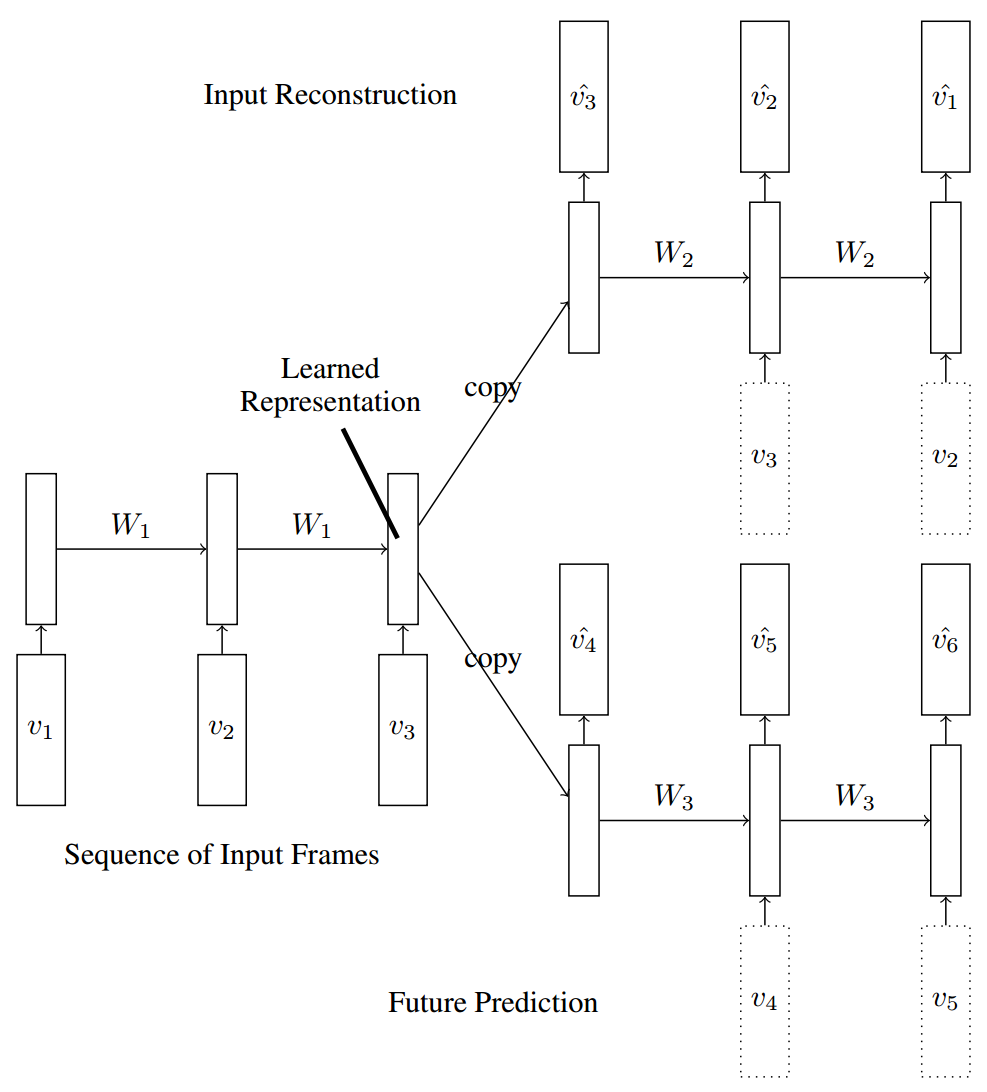
\includegraphics[width=0.7\textwidth]{img/unsupervised_learning_with_lstms_composite.png}
	\caption{Composite model for input reconstruction and future prediction \cite{unsupervised_learning_lstms}}
	\label{fig:stateofart:unsupervised_lstm_composite}
\end{figure}



\section{Machine Learning for Network Intrusion Detection}


Here provide an overview of the related state of art. Look for papers that are closest to the research you are doing
Suggestion: make a table with the related papers and compare them wrt to different criteria, for instance

\begin{itemize}
	\item Findings: What do they claim (main findings)
	\item Data: What data set they are using
	\item Methods: Which methods did they use?
	\item Reproducibility: Is it possible to reproduce the results? (e.g., is the data available? are all parameter settings provided? Is source code provided?)
	\item Relevance (How relevant is it for your work)
\end{itemize}


In the last paragraph explain how your work differs from the existing works.



\newpage
